\chapter{Implementacija i korisničko sučelje}
		\begin{flushleft}
		\section{Korištene tehnologije i alati}

			Komunikacija u timu realizirana je korištenjem aplikacija Whatsapp \footnote{https://whatsapp.com/} i Microsoft Teams \footnote{https://www.microsoft.com/en/microsoft-teams}. Za izradu UML dijagrama korišten je alat Astah Professional \footnote{https://astah.net/downloads/}, a kao sustav za upravljanje izvornim kodom Git \footnote{https://git-scm.com/}. Udaljeni repozitorij projekta dostupan je na web platformi GitLab \footnote{https://about.gitlab.com/}. 
		    Kao razvojno okruženje korišten je Microsoft Visual Studio Code \footnote{https://code.visualstudio.com/}. U backend dijelu aplikacije korišten je Express.js\footnote{https://expressjs.com/}, radni okvir za Node.js \footnote{https://nodejs.org/en/}. Express-om je riješeno {routanje}, tj. odgovaranje na korisničke upite i prikazivanje različitih dijelova aplikacije. 
            Za komunikaciju s bazom podataka korišten je Node.js klijent pg \footnote{https://www.pgadmin.org/}. U frontend dijelu aplikacije korišten je skriptni jezik HTML \footnote{https://hr.wikipedia.org/wiki/HTML}, CSS \footnote{https://en.wikipedia.org/wiki/CSS} i Bootstrap. Pri izradi dokumentacije korišten je alat Overleaf \footnote{https://www.overleaf.com} dostupan na internetu.
            \vspace*{\stretch{1.0}}
			
			\eject 
		
	
		\section{Ispitivanje programskog rješenja}
	
			\subsection{Ispitivanje komponenti}
			\text{Ispitivanje komponenti provedeno je koristeći Node.js frameworkove Mocha i Chai }
			
			\begin{figure}[hp]
                    \centering
                    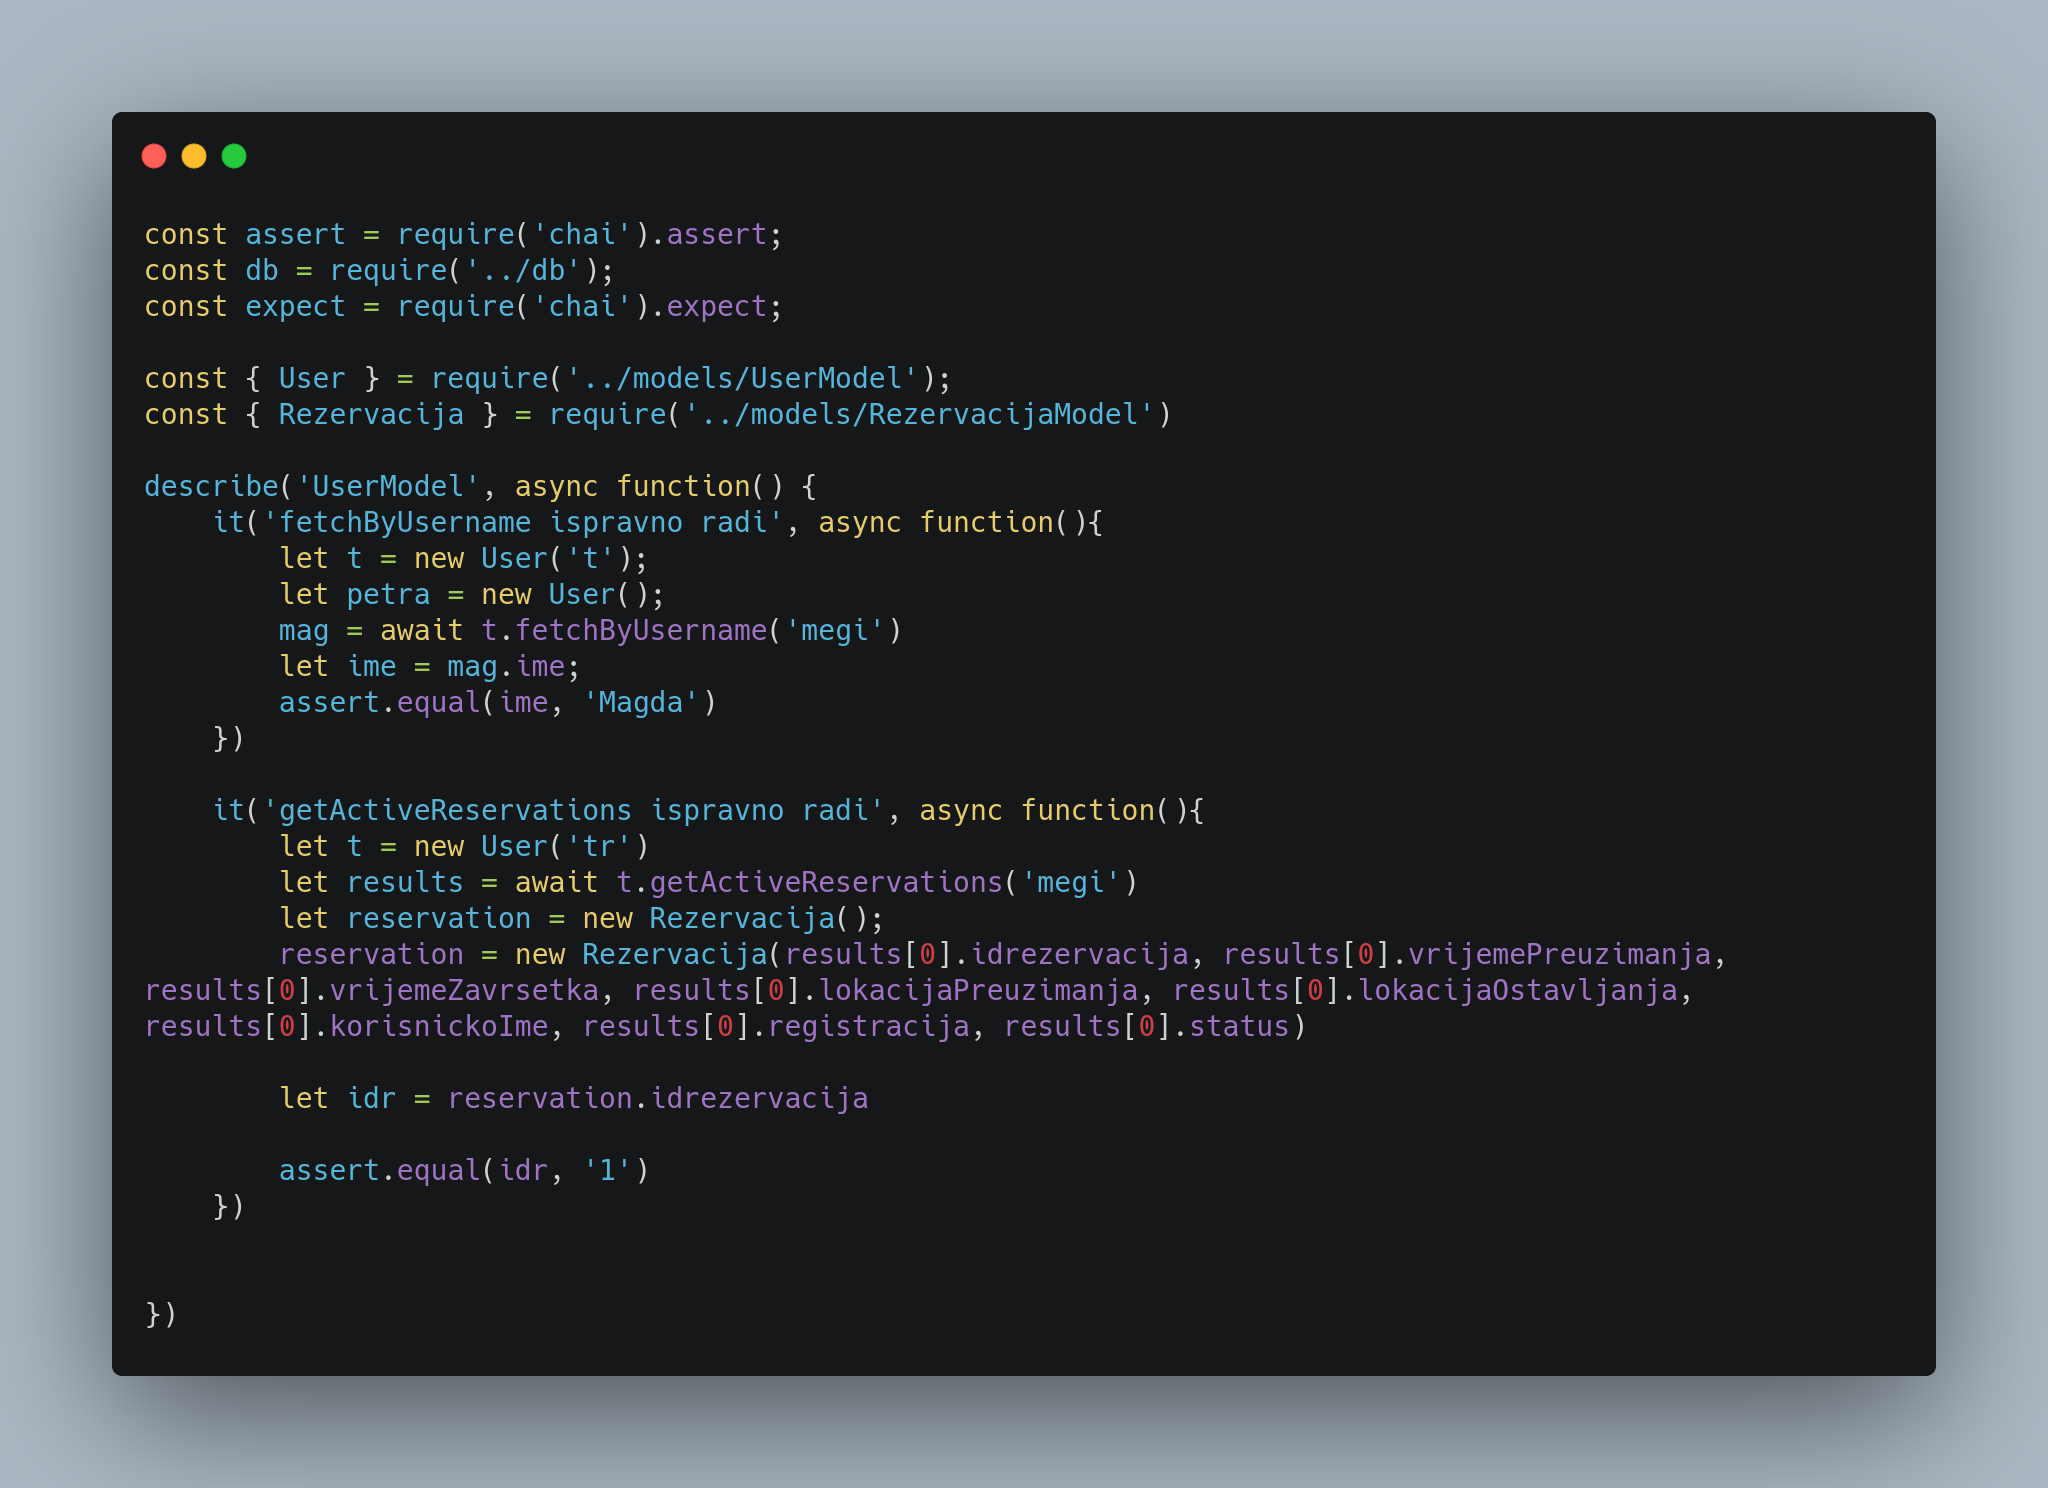
\includegraphics[width=15cm]{slike/UserModel.png}
                    \caption{Testiranje UserModela}
                    \label{fig:useCase-2}
                \end{figure}
			\eject 
			
	
			
			\begin{figure}[hp]
                    \centering
                    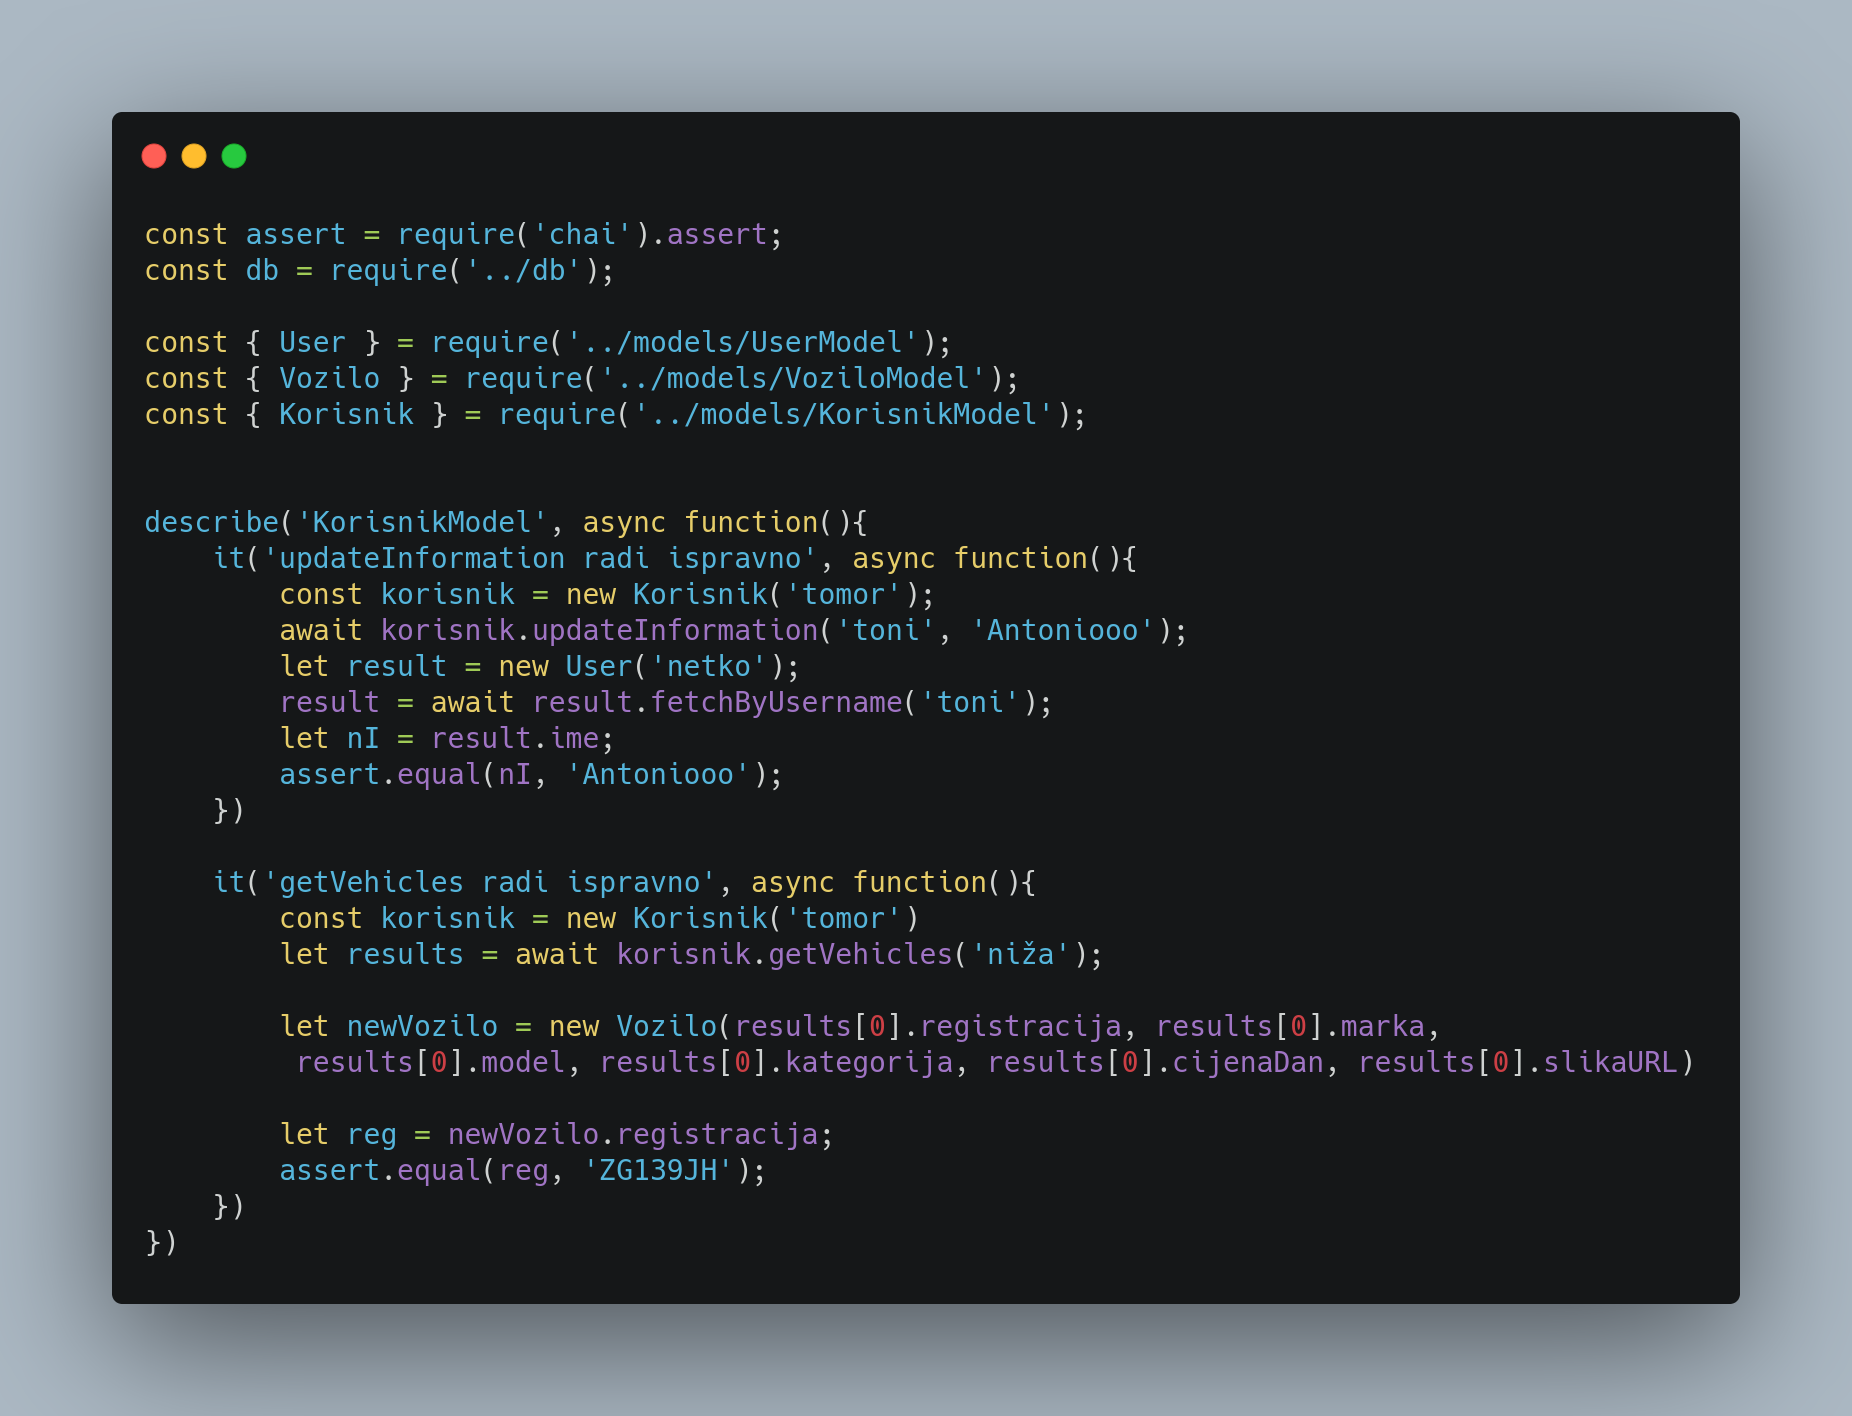
\includegraphics[width=15cm]{slike/KorisnikModel.png}
                    \caption{Testiranje KorisnikModela}
                    \label{fig:useCase-2}
                \end{figure}
			\eject 
			
			\begin{figure}[hp]
                    \centering
                    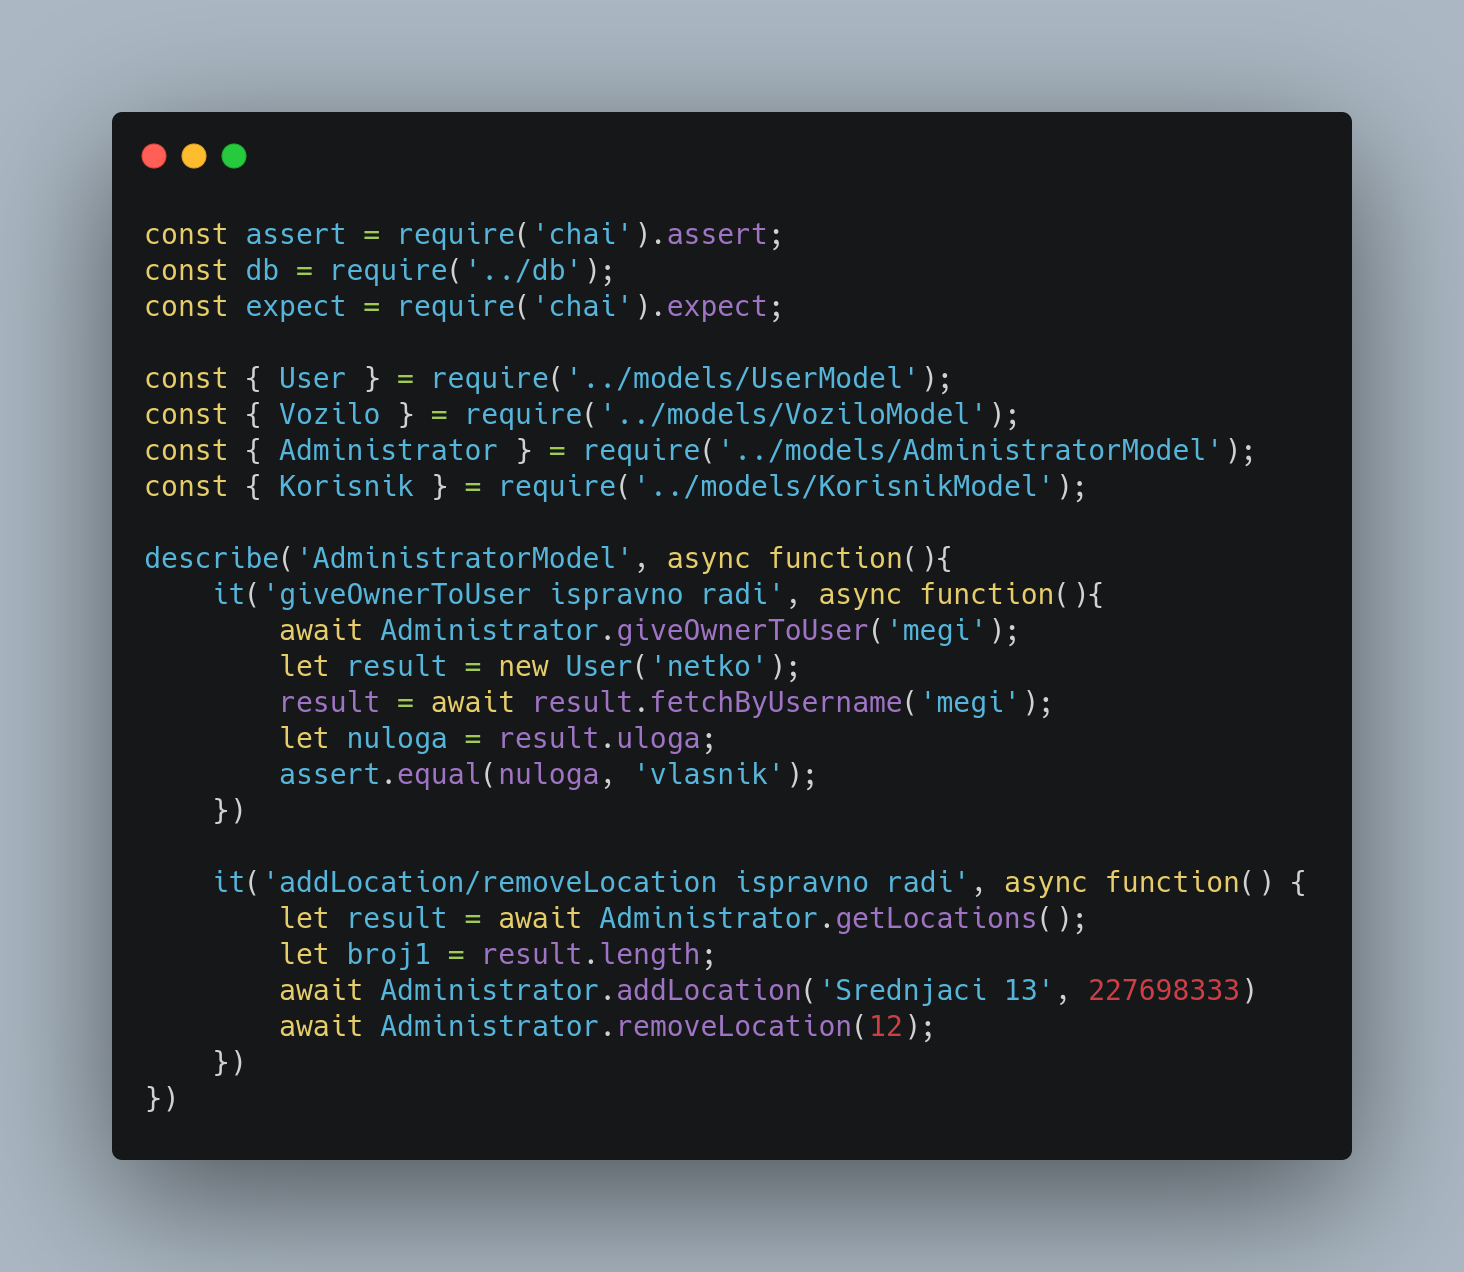
\includegraphics[width=15cm]{slike/AdministratorModel.png}
                    \caption{Testiranje AdministratorModela}
                    \label{fig:useCase-2}
                \end{figure}
			\eject 
			
			
			\begin{figure}[hp]
                    \centering
                    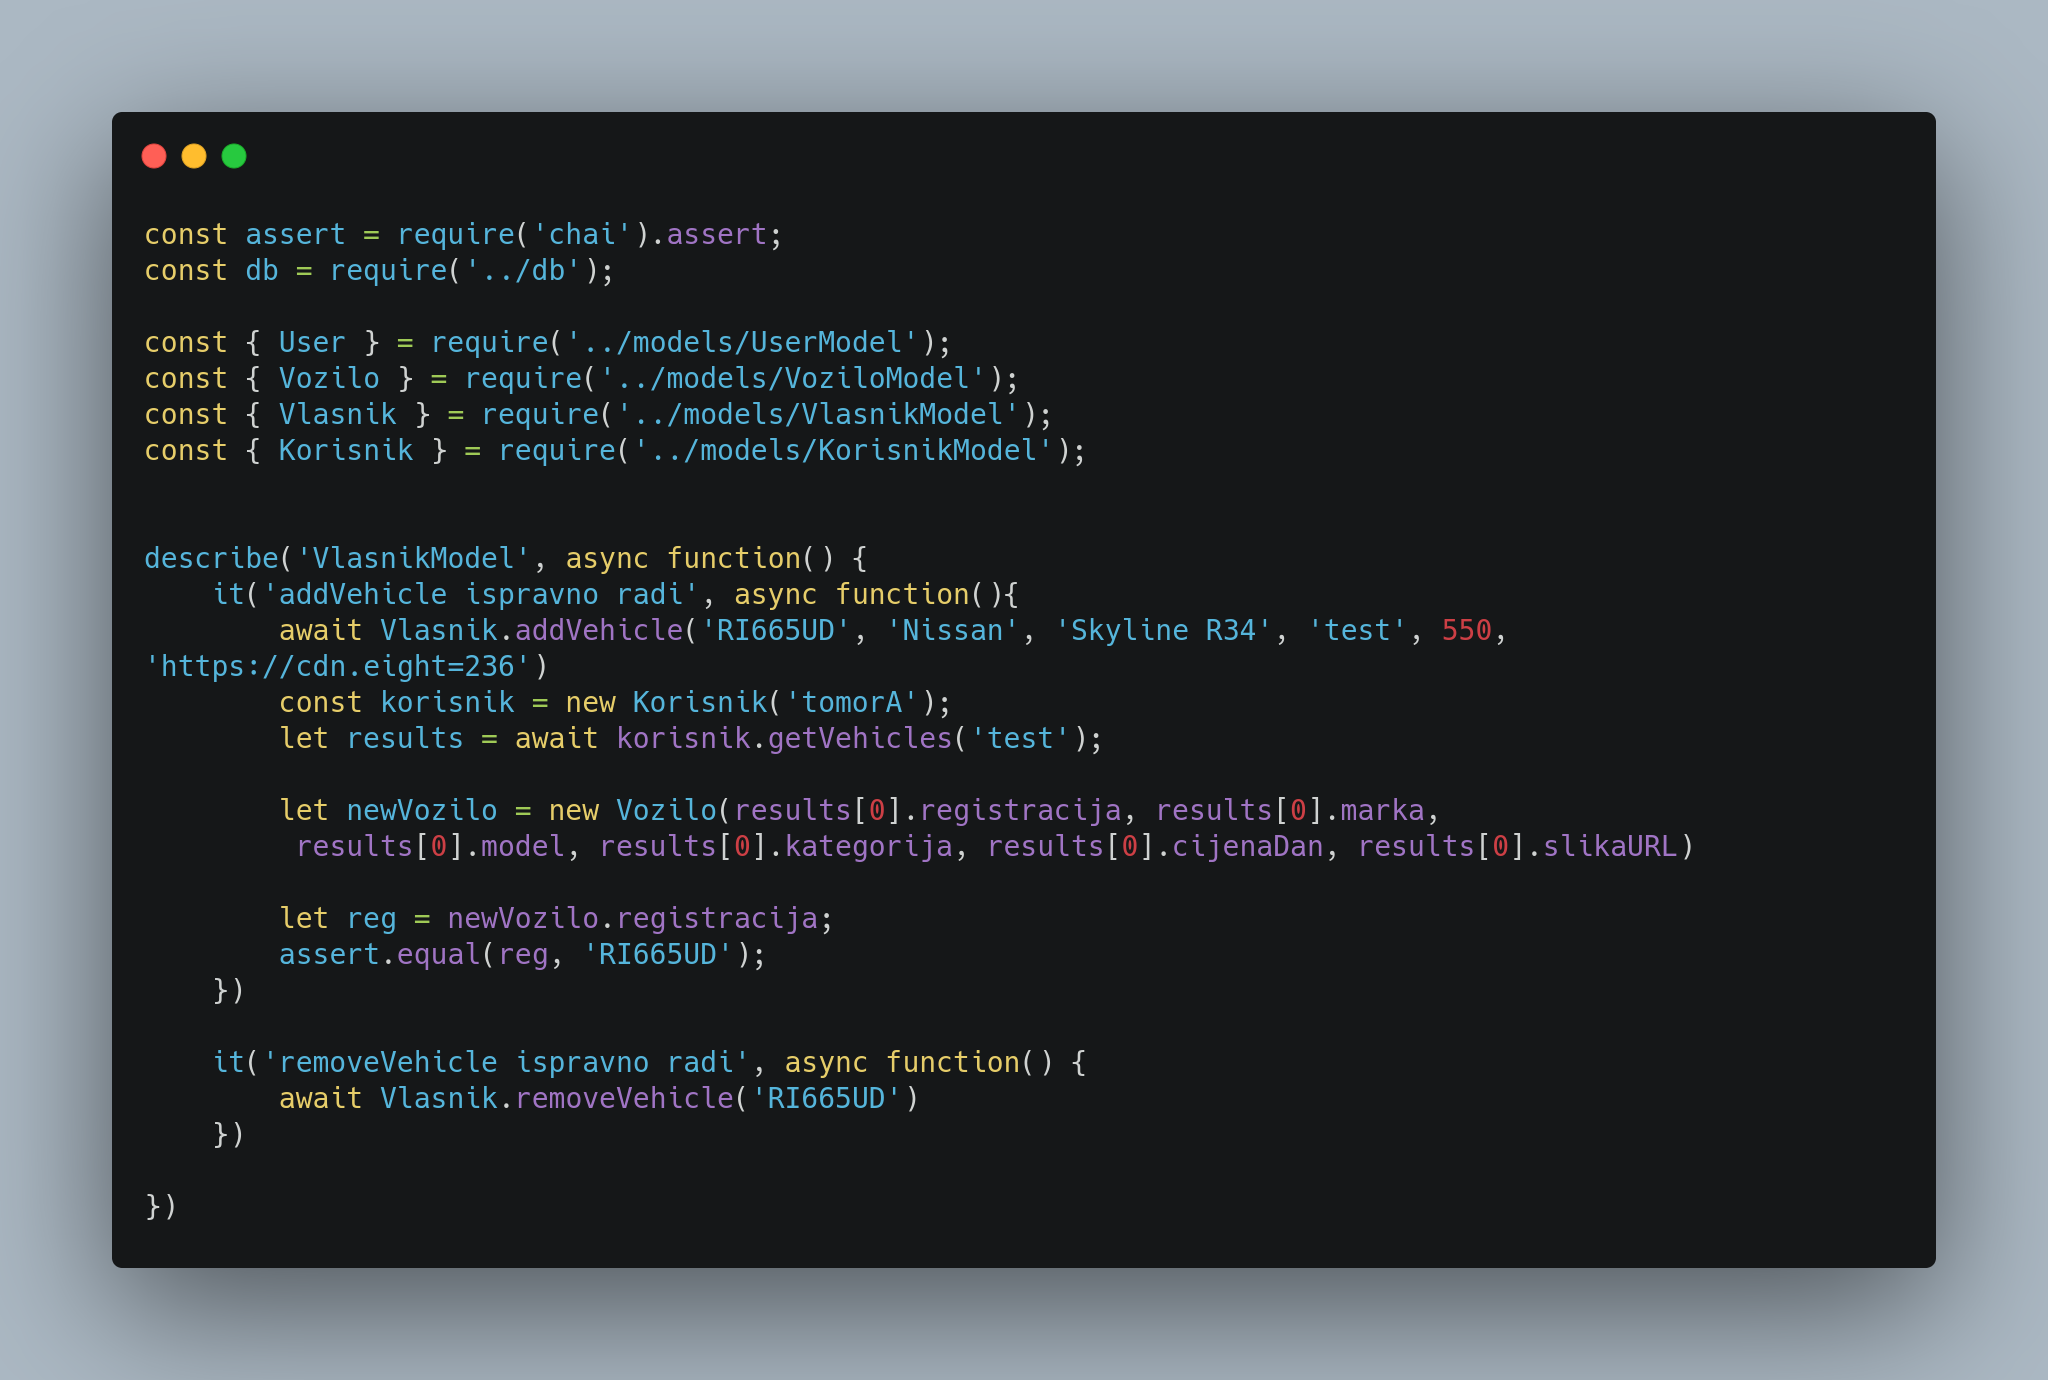
\includegraphics[width=15cm]{slike/VlasnikModel.png}
                    \caption{Testiranje VlasnikModela}
                    \label{fig:useCase-2}
                \end{figure}
			\eject 
			
			\begin{figure}[hp]
                    \centering
                    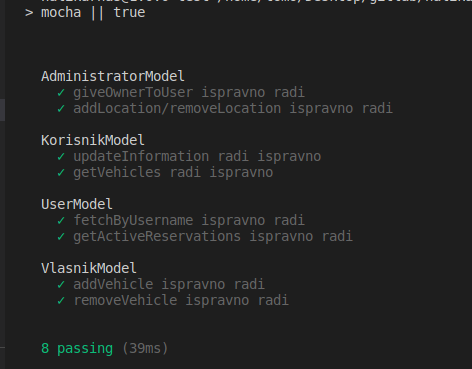
\includegraphics[width=15cm]{slike/rjesenjeeeee.png}
                    \caption{Rezultati testova}
                    \label{fig:useCase-2}
                \end{figure}
			\eject 
			
			
			
			\subsection{Ispitivanje sustava}
			    
			    \noindent{Ispitivanje sustava proveli smo koristeći Selenium WebDriver (\textit{https://selenium.dev/documentation/en/selenium-installation/}) unutar JUnit testova. Kodovi za ispitivanje ispravne i neisprave prijave dani su na slikama 5.6 i 5.7, a rezultati testa vidljivi su na slici 5.8.}
			
			\begin{figure}[hp]
                    \centering
                    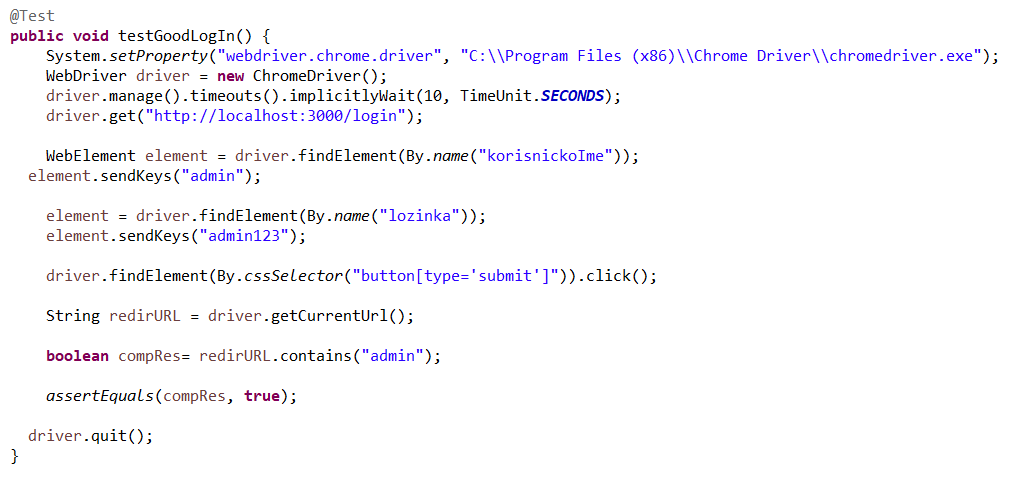
\includegraphics[width=15cm]{slike/koddobraprijava.png}
                    \caption{Kod ispravne prijave}
                    \label{fig:useCase-2}
                \end{figure}
			\eject
            
            \begin{figure}[hp]
                    \centering
                    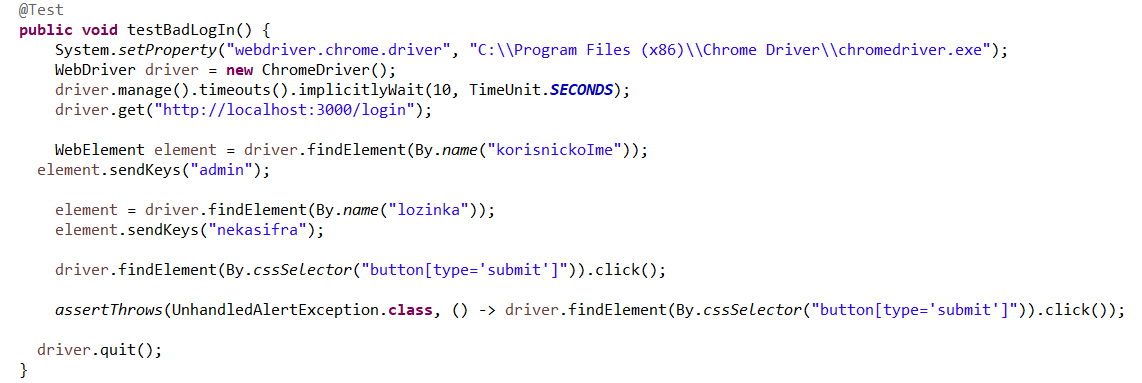
\includegraphics[width=15cm]{slike/kodlosaprijava.png}
                    \caption{Kod neispravne prijave}
                    \label{fig:useCase-2}
                \end{figure}
			\eject
			
			\begin{figure}[hp]
                    \centering
                    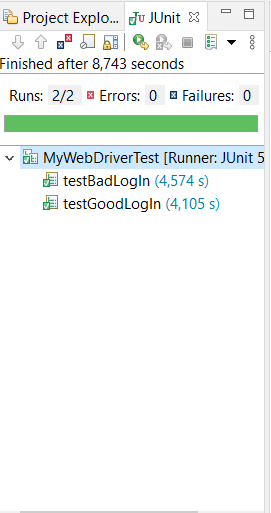
\includegraphics[width=15cm]{slike/logintests.png}
                    \caption{Rezultati testova}
                    \label{fig:useCase-2}
                \end{figure}
			\eject
			
			    \noindent{Kodovi za ispitivanje ispravne i neisprave pretrage vozila dani su na slikama 5.9 i 5.10, a rezultati testa vidljivi su na slici 5.11. Kod dobre pretrage nakon unosa datuma, klikom na gumb prikazuju nam se auti koji se mogu rezervirati. U slučaju unosa neispravnog datuma, stranica nas o tom obavještava pomoću alert box-a.}
			
			\begin{figure}[hp]
                    \centering
                    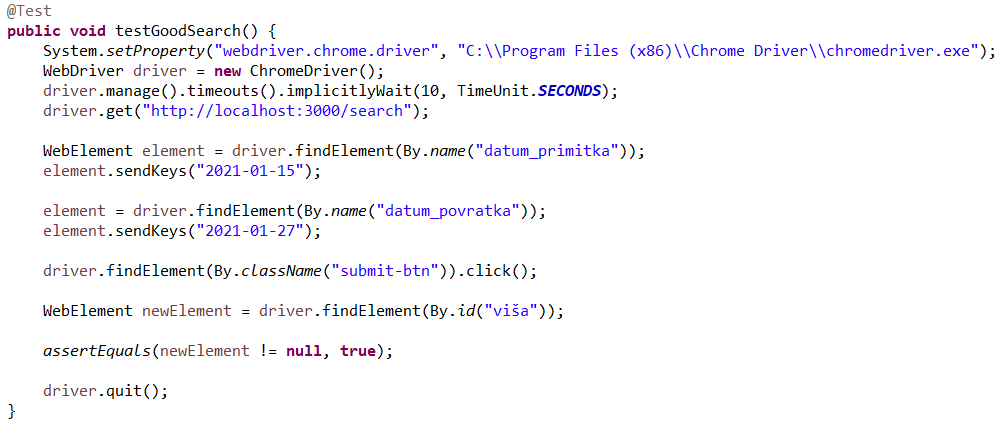
\includegraphics[width=15cm]{slike/koddobrapretraga.png}
                    \caption{Kod ispravne pretrage}
                    \label{fig:useCase-2}
                \end{figure}
			\eject
			
			\begin{figure}[hp]
                    \centering
                    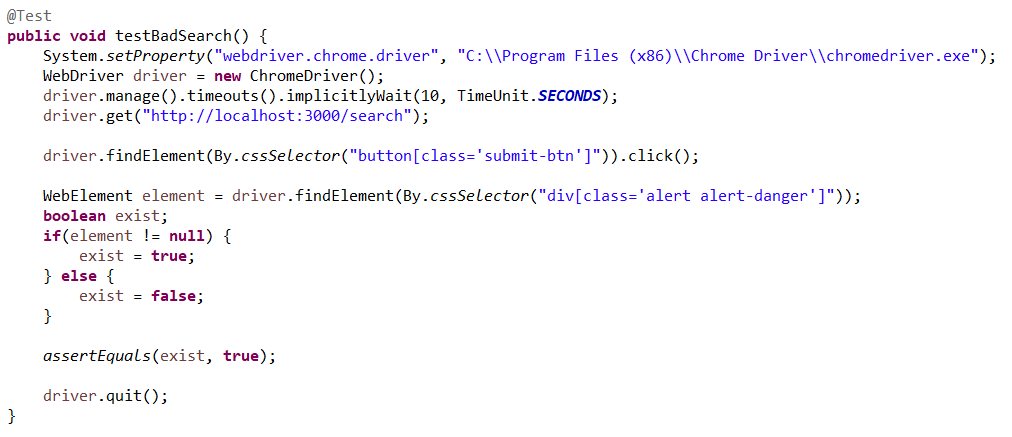
\includegraphics[width=15cm]{slike/kodlosapretraga.png}
                    \caption{Kod neispravne pretrage}
                    \label{fig:useCase-2}
                \end{figure}
			\eject
			
			\begin{figure}[hp]
                    \centering
                    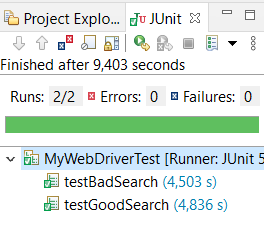
\includegraphics[width=15cm]{slike/searchtests.png}
                    \caption{Rezultati testova}
                    \label{fig:useCase-2}
                \end{figure}
			\eject
			
			\noindent{Kodovi za ispitivanje uspješne i neuspješne lozinke dani su na slikama 5.12 i 5.13, a rezultati testova dani su na slikama 5.14 i 5.15. U slučaju uspješne promjene lozinke, korisnik se preusmjerava na početnu stranicu, dok u slučaju neuspješne promjene korisnik dobije poruku o neuspjehu.}
			
			\begin{figure}[hp]
                    \centering
                    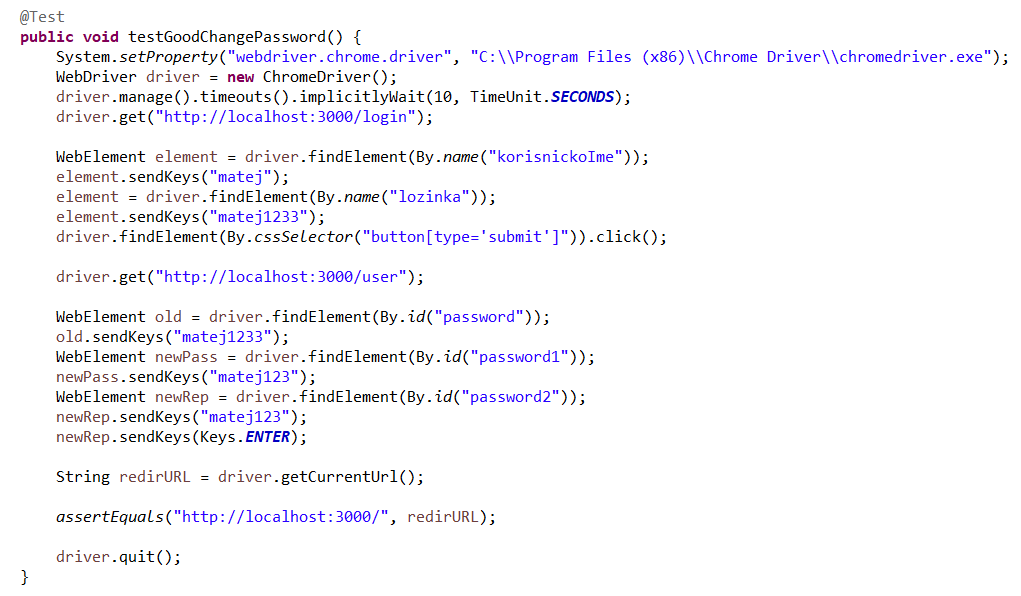
\includegraphics[width=15cm]{slike/koddobrapromjenalozinke.png}
                    \caption{Uspješna promjena lozinke}
                    \label{fig:useCase-2}
                \end{figure}
			\eject
			
			\begin{figure}[hp]
                    \centering
                    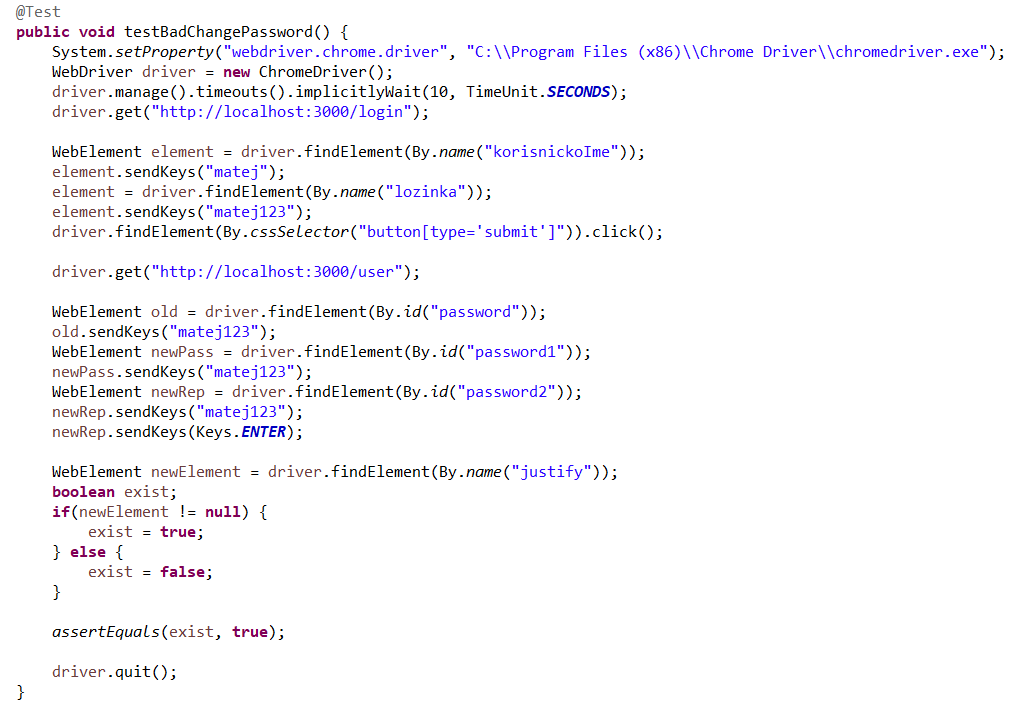
\includegraphics[width=15cm]{slike/kodlosapromjenalozinke.png}
                    \caption{Neuspješna promjena lozinke}
                    \label{fig:useCase-2}
                \end{figure}
			\eject
			
			\begin{figure}[hp]
                    \centering
                    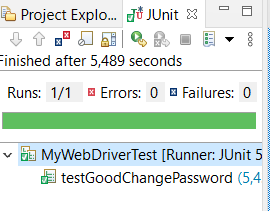
\includegraphics[width=15cm]{slike/passwordgood.png}
                    \caption{Rezultat testa uspješne promjene lozinke}
                    \label{fig:useCase-2}
                \end{figure}
			\eject
			
			\begin{figure}[hp]
                    \centering
                    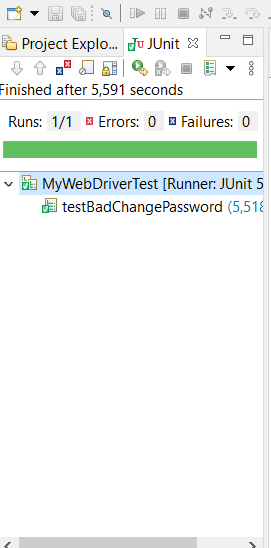
\includegraphics[width=15cm]{slike/passwordbad.png}
                    \caption{Rezultat testa neuspješne promjene lozinke}
                    \label{fig:useCase-2}
                \end{figure}
			\eject
			
			\noindent{Kodovi za ispitivanje rezervacije vozila dani su na slikama 5.16 i 5.17, a rezultati testova dani su na slikama 5.18 i 5.19. Prijavljeni korisnik može rezervirati auto, dok neprijavljeni korisnik ne može zato što mu gumb za rezervaciju nije vidljiv.}
			
			\begin{figure}[hp]
                    \centering
                    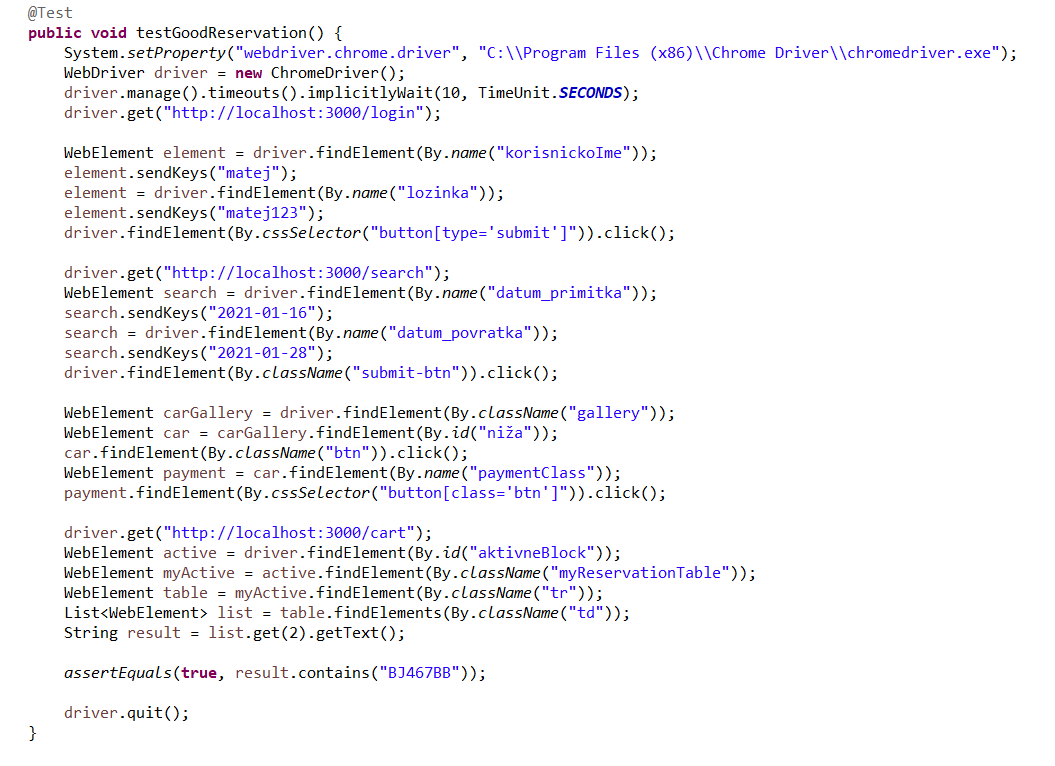
\includegraphics[width=15cm]{slike/koddobrarezervacija.png}
                    \caption{Uspješna rezervacija}
                    \label{fig:useCase-2}
                \end{figure}
			\eject
			
			\begin{figure}[hp]
                    \centering
                    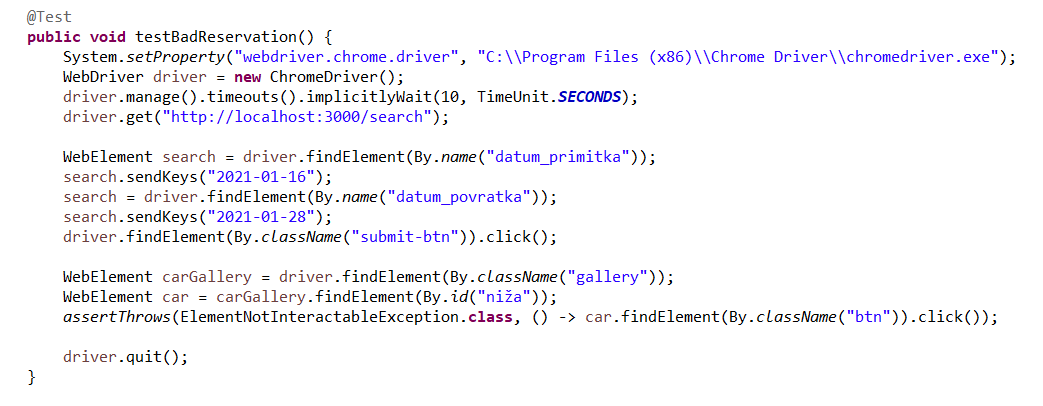
\includegraphics[width=15cm]{slike/kodlosarezervacija.png}
                    \caption{Neuspješna rezervacija}
                    \label{fig:useCase-2}
                \end{figure}
			\eject
			
			\begin{figure}[hp]
                    \centering
                    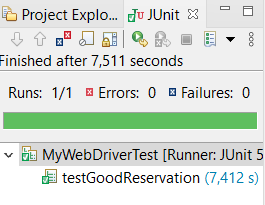
\includegraphics[width=15cm]{slike/reservationgood.png}
                    \caption{Rezultat testa uspješne rezervacije}
                    \label{fig:useCase-2}
                \end{figure}
			\eject
			
			\begin{figure}[hp]
                    \centering
                    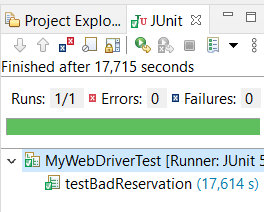
\includegraphics[width=15cm]{slike/reservationbad.png}
                    \caption{Rezultat testa neuspješne rezervacije}
                    \label{fig:useCase-2}
                \end{figure}
			\eject
			
			\eject 
		
		
		\section{Dijagram razmještaja}
			
			
			
			  \noindent Dijagram razmještaja prikazuje radno okruženje sklopovlja i programske potpore. Na poslužiteljskom računalu se nalazi poslužitelj za bazu podataka i web poslužitelj. Na klijentskom računalu koristi se web preglednik kako bi se pristupilo web alikaciji. Komunikacija između računala korisnika i poslužitelja odvija se preko HTTP veze.
			
			\begin{figure}[hp]
                    \centering
                    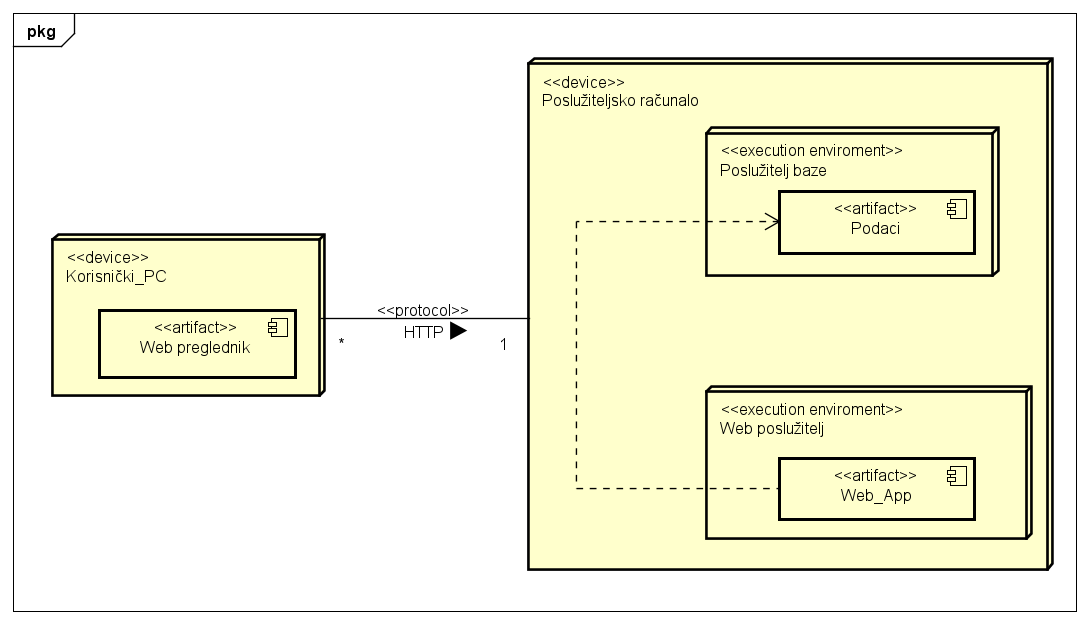
\includegraphics[width=16cm]{slike/Dijagram_razmjestaja.png}
                    \caption{Dijagram razmještaja}
                    \label{fig:DR_01}
                \end{figure}
			    
			\eject 
			
		
		\section{Upute za puštanje u pogon}
		
			\subsection{Stvaranje servera}
			
	        \begin{enumerate}
			
			
			\item Stvoriti korisnički račun na GitHub platformi. Na GitHubu se nudi mogućnost posebne ponude za studente, koju želimo iskoristiti. Potrebno je kopirati kod kako bismo ostvarili popust pri podizanju naše web stranice na server pomoću DigitalOcean platforme.
			
			\item Stvoriti korisnički račun na DigitalOcean platformi i unijeti kopirani kod za popust. 
			
			\item  Stvoriti novi droplet na lokaciji Frankfurt
			 pretplate 5\$ mjesečno. 
			
		\end{enumerate}
		
		\subsection{Postavljanje korisnika na serveru}
	    \begin{enumerate}
	       	\item Pokrenemo Command Prompt i pokrenemo sljedeće naredbe za korisnika josip
			\item ssh root@46.101.144.41
			\item Unesemo i pokrenemo naredbu adduser josip  
			\item usermod -aG sudo josip
			\item usermod -aG sudo josip
			\item ufw allow OpenSSH
			\item ufw enable
			\item ufw status
			\item mkdir /home/josip/.ssh
			\item nano /home/josip/.ssh/authorized\_keys
			\item chmod -R go= ~/.ssh
			\item chown -R josip:josip ~/.ssh
		\end{enumerate}
	        
	   \subsection{Postavljanje domene}
	   \begin{enumerate}
	        \item Otvoriti DuckDNS i logirati se sa GitHub profilom
	        \item Stvoriti domenu po želji (odabrana: halikarnas-autos.duckdns.org)
	        \item Kopirati IPv4 dropleta s DigitalOcean portala u DuckDNS portal
	        \item U DO portali otići u Networking i dodati domenu navedenu u DuckDNS portalu
	        \item Dodati A zapis za domenu * i www inačicu
	   \end{enumerate}
	   
	   \subsection{Postavljanje nginxa}
	   \begin{enumerate}
	        \item sudo apt update
	        \item sudo apt install nginx
	        \item sudo ufw app list (je li registrirao nginx)
	        \item sudo ufw allow 'Nginx HTTP'
	        \item sudo ufw status (provjera je li omogućio nginx)
	        \item systemctl status nginx (mora pisati active)
	        \item curl http://46.101.144.41 (provjera javlja li “welcome to nginx”)
	        \item curl http://halikarnas-autos.duckdns.org (provjera javlja li “welcome to nginx”)
	   \end{enumerate}
	   
	   \subsection{Postavljanje nginx blokova}
	   \begin{enumerate}
	        \item sudo mkdir -p /var/www/halikarnas-autos.duckns.org/html
	        \item sudo chown -R $USER:$USER /var/www/halikarnas-autos.duckns.org/html
	        \item sudo chmod -R 755 /var/www/halikarnas-autos.duckns.org
	        \item nano /var/www/halikarnas-autos.duckns.org/html/index.html (zaljepiti text klasične html stranice)
	        \item sudo nano /etc/nginx/sites-available/halikarnas-autos.duckns.org (zaljepiti text konfiguracije)
	        \item sudo ln -s /etc/nginx/sites-available/halikarnas-autos.duckns.org /etc/nginx/sites-enabled/
	        \item sudo nano /etc/nginx/nginx.conf (odkomentiraj \# kod linije sa brojem 64)
	        \item sudo rm -r /etc/nginx/sites-available/default (ako treba i iz sites-enabled mape)
	        \item sudo nginx -t (provjera je li konfiguracija točna na suho)
	        \item ako je sve u redu, pokreni: sudo systemctl restart nginx
	   \end{enumerate}

    \subsection{Secure nginx}
	   \begin{enumerate}
	        \item sudo apt install certbot python3-certbot-nginx
	        \item sudo ufw allow 'Nginx Full'
	        \item sudo certbot --nginx -d halikarnas-autos.duckns.org -d www.halikarnas-autos.duckns.org
	        \item sudo systemctl status certbot.timer (mora biti active)
	        \item sudo service nginx restart (kako bi se zabilježile promjene)
	   \end{enumerate}
	   
	   \subsection{Postavljanje baze}
	   \begin{enumerate}
	        \item sudo apt update
	        \item sudo apt install postgresql postgresql-contrib
	        \item sudo -i -u postgres pa psql (ili sudo -u postgres psql za bazu)
	        \item createdb autos (import ne radimo jer imamo seeder.js)
	        \item ALTER USER postgres WITH PASSWORD 'new\_password'; (navesti istu lozinku kao u postavkama index.js za spajanje, ako je potrebno mijenjati)
	   \end{enumerate}
	   
	   \subsection{Postavljanje Node.js}
	   \begin{enumerate}
	        \item cd \textasciitilde{} (tilda)
	        \item curl -sL https://deb.nodesource.com/setup\_14.x -o nodesource\_setup.sh
	        \item sudo bash nodesource\_setup.sh
	        \item sudo apt install nodejs
	        \item sudo apt install build-essential
	        \item napraviti git clone https://gitlab.com/josip.hrvatic/halikarnas.git u mapu /var/www/halikarnas-autos.duckns.org/html
	        \item provjeriti jesu li podaci za prijavu u bazu u skladu sa pravim podacima na serveru (zato postoje upute za mijenjanje lozinke u koraku iznad)
	        \item u nginx konfiguraciji postaviti naredbu na listen:80 ali u odjeljku location ima naredbu proxy\_pass ‘halikarnas-autos.duckns.org:3000’ jer je takav port naveden u server.js
	   \end{enumerate}
	   
	   \subsection{Postavljanje beskonačnog procesa}
	   \begin{enumerate}
	        \item sudo npm install pm2@latest -g
	        \item pm2 start server.js
	   \end{enumerate}
	   
	   \subsection{Kontinuirano dodavanje promjena na server}
	   \begin{enumerate}
	        \item ssh josip@halikarnas-autos.duckdns.org
	        \item cd /var/www/halikarnas-autos.duckdns.org/html/halikarnas
	        \item git pull origin develop (ili master, ovisi na kojoj grani je produkcija)
	        \item pm2 restart server (kako bi se promjene vidjele)
	   \end{enumerate}
	\end{flushleft}

